\documentclass[twocolumn,twoside,10pt,a4paper]{article}

\usepackage[english]{babel}  % portuguese
\usepackage{graphicx}           % images: .png or .pdf w/ pdflatex; .eps w/ latex

%% For iso-8859-1 (latin1), comment next line and uncomment the second line
\usepackage[utf8]{inputenc}

\usepackage{times}              % PS fonts
\usepackage[T1]{fontenc}        % T1 fonts
%\usepackage{lastpage}           % to have lastpage in headers
\usepackage{url}                % urls

% geometry package
\usepackage[outer=20mm,inner=30mm,vmargin=20mm,includehead,includefoot,headheight=15pt]{geometry}

%% space between columns
\columnsep 10mm

% avoid widows and orphans
\clubpenalty=300
\widowpenalty=300

\usepackage{listings}
\lstdefinestyle{xml}{
	language=XML,
	extendedchars=true,
	inputencoding=latin1,
	tabsize=4,
	showstringspaces=false,
	basicstyle=\scriptsize,
	keywordstyle=\ttfamily\color{blue},
	stringstyle=\ttfamily\color{orange},
	identifierstyle=\ttfamily,
	commentstyle=\ttfamily\color{darkred},
	morecomment=[s][\ttfamily\color{javadoc}]{/**}{*/},
	numbers=left
}

\usepackage[pdftex]{hyperref}
\hypersetup{%
    a4paper = true,              % use A4 paper
    bookmarks = true,            % make bookmarks
    colorlinks = true,           % false: boxed links; true: colored links
    pdffitwindow = false,        % page fit to window when opened
    pdfpagemode = UseNone,       % do not show bookmarks
    pdfpagelayout = SinglePage,  % displays a single page
    pdfpagetransition = Replace, % page transition
    linkcolor=blue,              % hyperlink colors
    urlcolor=blue,
    citecolor=blue,
    anchorcolor=green
}

\usepackage{indentfirst}       % indent also 1st paragraph

\pagestyle{myheadings}         % Option to put page headers
\markboth{{\small\it xml2json}}
{{\small\it Group 08, \today}}

%\hyphenation{}                  % explicit hyphenation

% entities
\newcommand{\class}[1]{{\normalfont\slshape #1\/}}

\title{xml2json}

\author{João Gradim\\
\small Faculdade de Engenharia da Universidade do Porto,\\[-0.8ex]
\small R.\ Dr.\ Roberto Frias, 4200-465 Porto\\[-0.8ex]
\small \texttt{ei05030@fe.up.pt}\\
\and
Nuno Polónia\\
\small Faculdade de Engenharia da Universidade do Porto,\\[-0.8ex]
\small R.\ Dr.\ Roberto Frias, 4200-465 Porto\\[-0.8ex]
\small \texttt{ei05037@fe.up.pt}
}

\date{\today}

\begin{document}

\maketitle
\thispagestyle{plain}

\begin{abstract}

\end{abstract}

\section{Introduction}\label{sec:intro}
On the newly programmable Web, mashups are flourishing. Designers create mashups by combining components of existing Web sites and applications \cite{maximilien}.
Using API\'s

\section{Objectives}\label{sec:objectives}

\section{User Requirements}\label{sec:user-requirements}

\section{Architecture}\label{sec:architecture}

xml2json acts primarily as a proxy that translates an XML document to a JSON representation. As such

\begin{figure}[h]
\centering
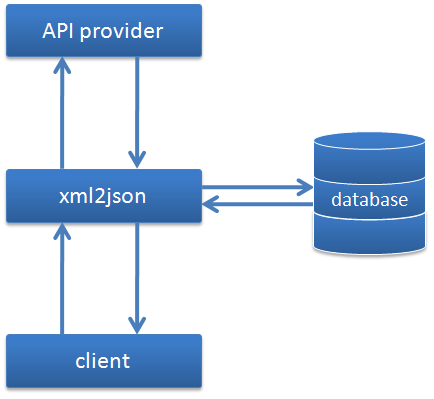
\includegraphics[width=80mm]{images/arch.png}
\caption{System Architecture}
\label{fig:system_arch}
\end{figure}

\section{Results}\label{sec:results}

\section{Final Remarks}\label{sec:final-remarks}

%% auto bibliographic list
\renewcommand{\bibname}{References}
\bibliographystyle{unsrt-pt}
\bibliography{lapd3}

\end{document}

